\subsection{Evaluating the Overhead of \texttt{PQ::moveHead()} and \texttt{PQ::chopHead()}}
\label{Sec-Eval-Move}

Maintaining separate skiplists for the sequential and the parallel part of the priority queue is beneficial for the overall throughput, but adds some overhead, which we quantify in this section. 
The number of elements that become part of the sequential skiplist changes dynamically based on the observed mix of operations. This adaptive behavior helps reduce the number of \texttt{moveHead()} and \texttt{chopHead()} operations required.  
Table~\ref{fig:sparc_headmove} shows the percentage of the number of head-moving operations out of the total number of \texttt{PQ::removeMin()} operations for different mixes of \texttt{PQ::add()} and \texttt{PQ::removeMin()} operations. The head-moving operations are rarely called due to the priority queue's adaptive behavior. 

\begin{table}[htb]
  \centering
	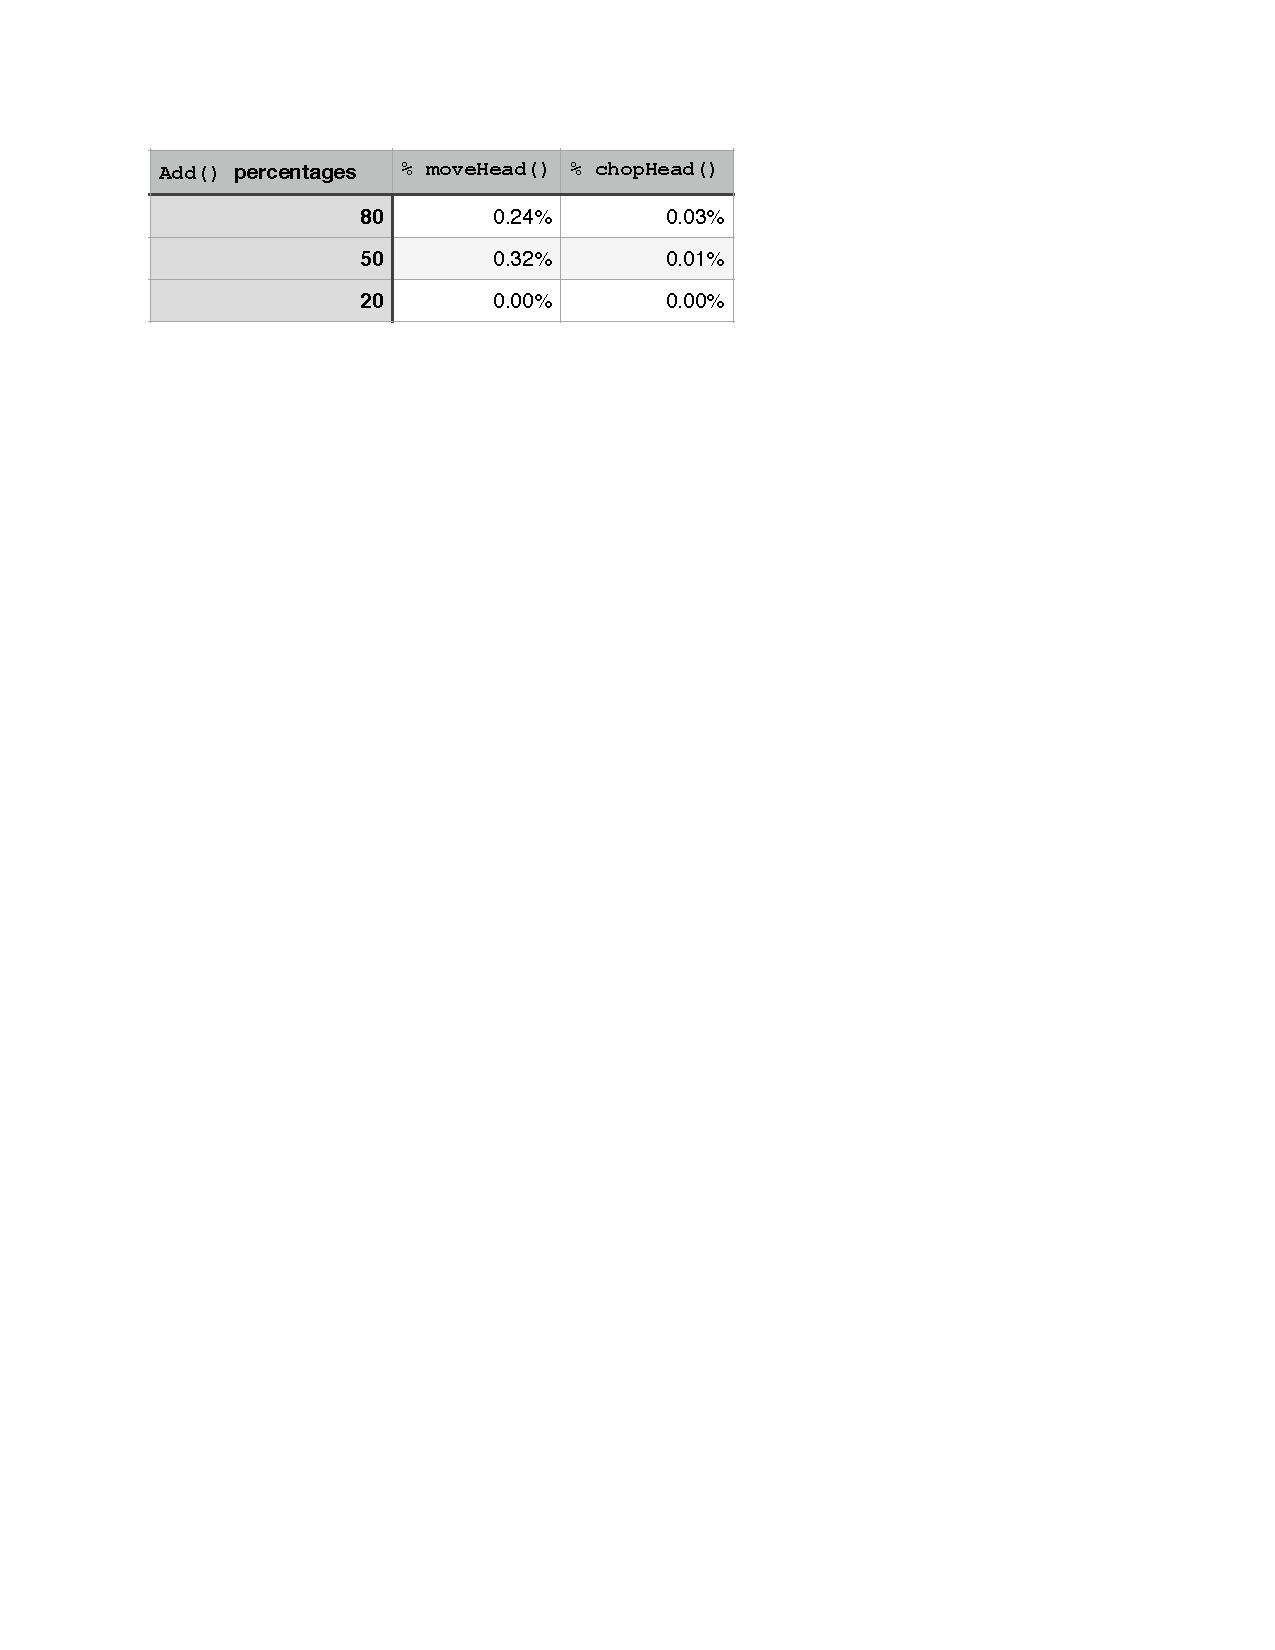
\includegraphics[width=0.65\textwidth]{img/sparc-stats-headmove.pdf}
	\caption{The number of head-moving operations as a percentage of the total number of \texttt{PQ::removeMin()} operations, considering different \texttt{add()} and \texttt{removeMin()} mixes.}
\label{fig:sparc_headmove}
\end{table}
